%% Copyright (C) 2019 Turysaz, Bitbonk
\documentclass{beamer}

%% Copyright (C) 2019 Turysaz, Bitbonk

\usepackage[utf8]{inputenc}
\usepackage[T1]{fontenc}
\usepackage[english]{babel}

\usepackage{todonotes}

%% packages needed by DarkConsole theme
\usepackage{xcolor}
\usepackage{pgf}
\usepackage{droidsans}
\usepackage{fvextra}
\usepackage{upquote}
\usepackage{slantsc}
%\usepackage{minted} %% needs shell escaping...
%\usepackage{ifplatform} %% needs shell escaping...
\usepackage{xstring}
\usepackage{framed}

\usetheme{DarkConsole}

\usepackage{pdfpcnotes}

\usepackage{caption}
\captionsetup[figure]{labelformat=empty}

\newcommand{
    \emojiLarge}[1]{
    \includegraphics[width=2cm]{../3rd-party/coloremoji/emoji_images/hires/#1.pdf}}

\newcommand{
    \emojiMedium}[1]{
    \includegraphics[width=1cm]{../3rd-party/coloremoji/emoji_images/hires/#1.pdf}}


\newcommand{
    \emojiSmall}[1]{
    \includegraphics{../3rd-party/coloremoji/emoji_images/hires/#1.pdf}}

\newcommand{\emojiCheck}{\emojiSmall{2705}}
\newcommand{\emojiFail}{\emojiSmall{1F6AB}}

%\newcommand{\says}[1]{\note{\huge{Says: \alert{#1}}}}
\newcommand{\says}[1]{\pnote{Says: #1}}



%% variables for koma title page
\author{\{@turysaz, @bitbonk\}}
\title{\Huge{Knit Rider}\\
    \large{Bring that 80s knitting machine to the 21st century!}
}

\date{\today{}}

\begin{document}

\maketitle

\begin{frame}{init}
      So we had an old knitting machine...
\end{frame}

%% photos of
%% - whole machine
%% - Nadelbett
%% - Schlitten
%% - E-Schlitten
%% - Demo-Bild aus Flyer
%% - Computer (Tastenfeld)

\begin{frame}{init}
    ...but the best thing is...\pause
    \begin{figure}
        \missingfigure{serial interface}
        \caption{it has a serial interface}
    \end{figure}
\end{frame}

\begin{frame}{the electronics}
    \begin{itemize}
        \item keypad
        \item manual programming
        \item data interface
    \end{itemize}
\end{frame}

\begin{frame}{the idea}
    \begin{enumerate}[<+->]
        \item Take a photo!
        \item Image processing!
        \item Do \_all\_ the soldering!
        \item Speak the protocol!
        \item Knit your face!
    \end{enumerate}
\end{frame}

\begin{frame}{the project architecture}
    \begin{figure}
        \missingfigure{the architecture}
    \end{figure}
\end{frame}

\begin{frame}{the different projects}
    \begin{description}[<+->]
        \item [knitt] the machine
        \item [michael] the driver
        \item [devon] pulling the strings
    \end{description}
\end{frame}

\begin{frame}{progress}
    \begin{enumerate}
        \item project name \pause (x) \pause
        \item github repos \pause (x) \pause
        \item logo \pause (x) \pause
        \item knit manually \pause (x) \pause
        \item power on ...! \pause
    \end{enumerate}
    ... \pause ...
\end{frame}

\begin{frame}{progress}
    \begin{figure}
        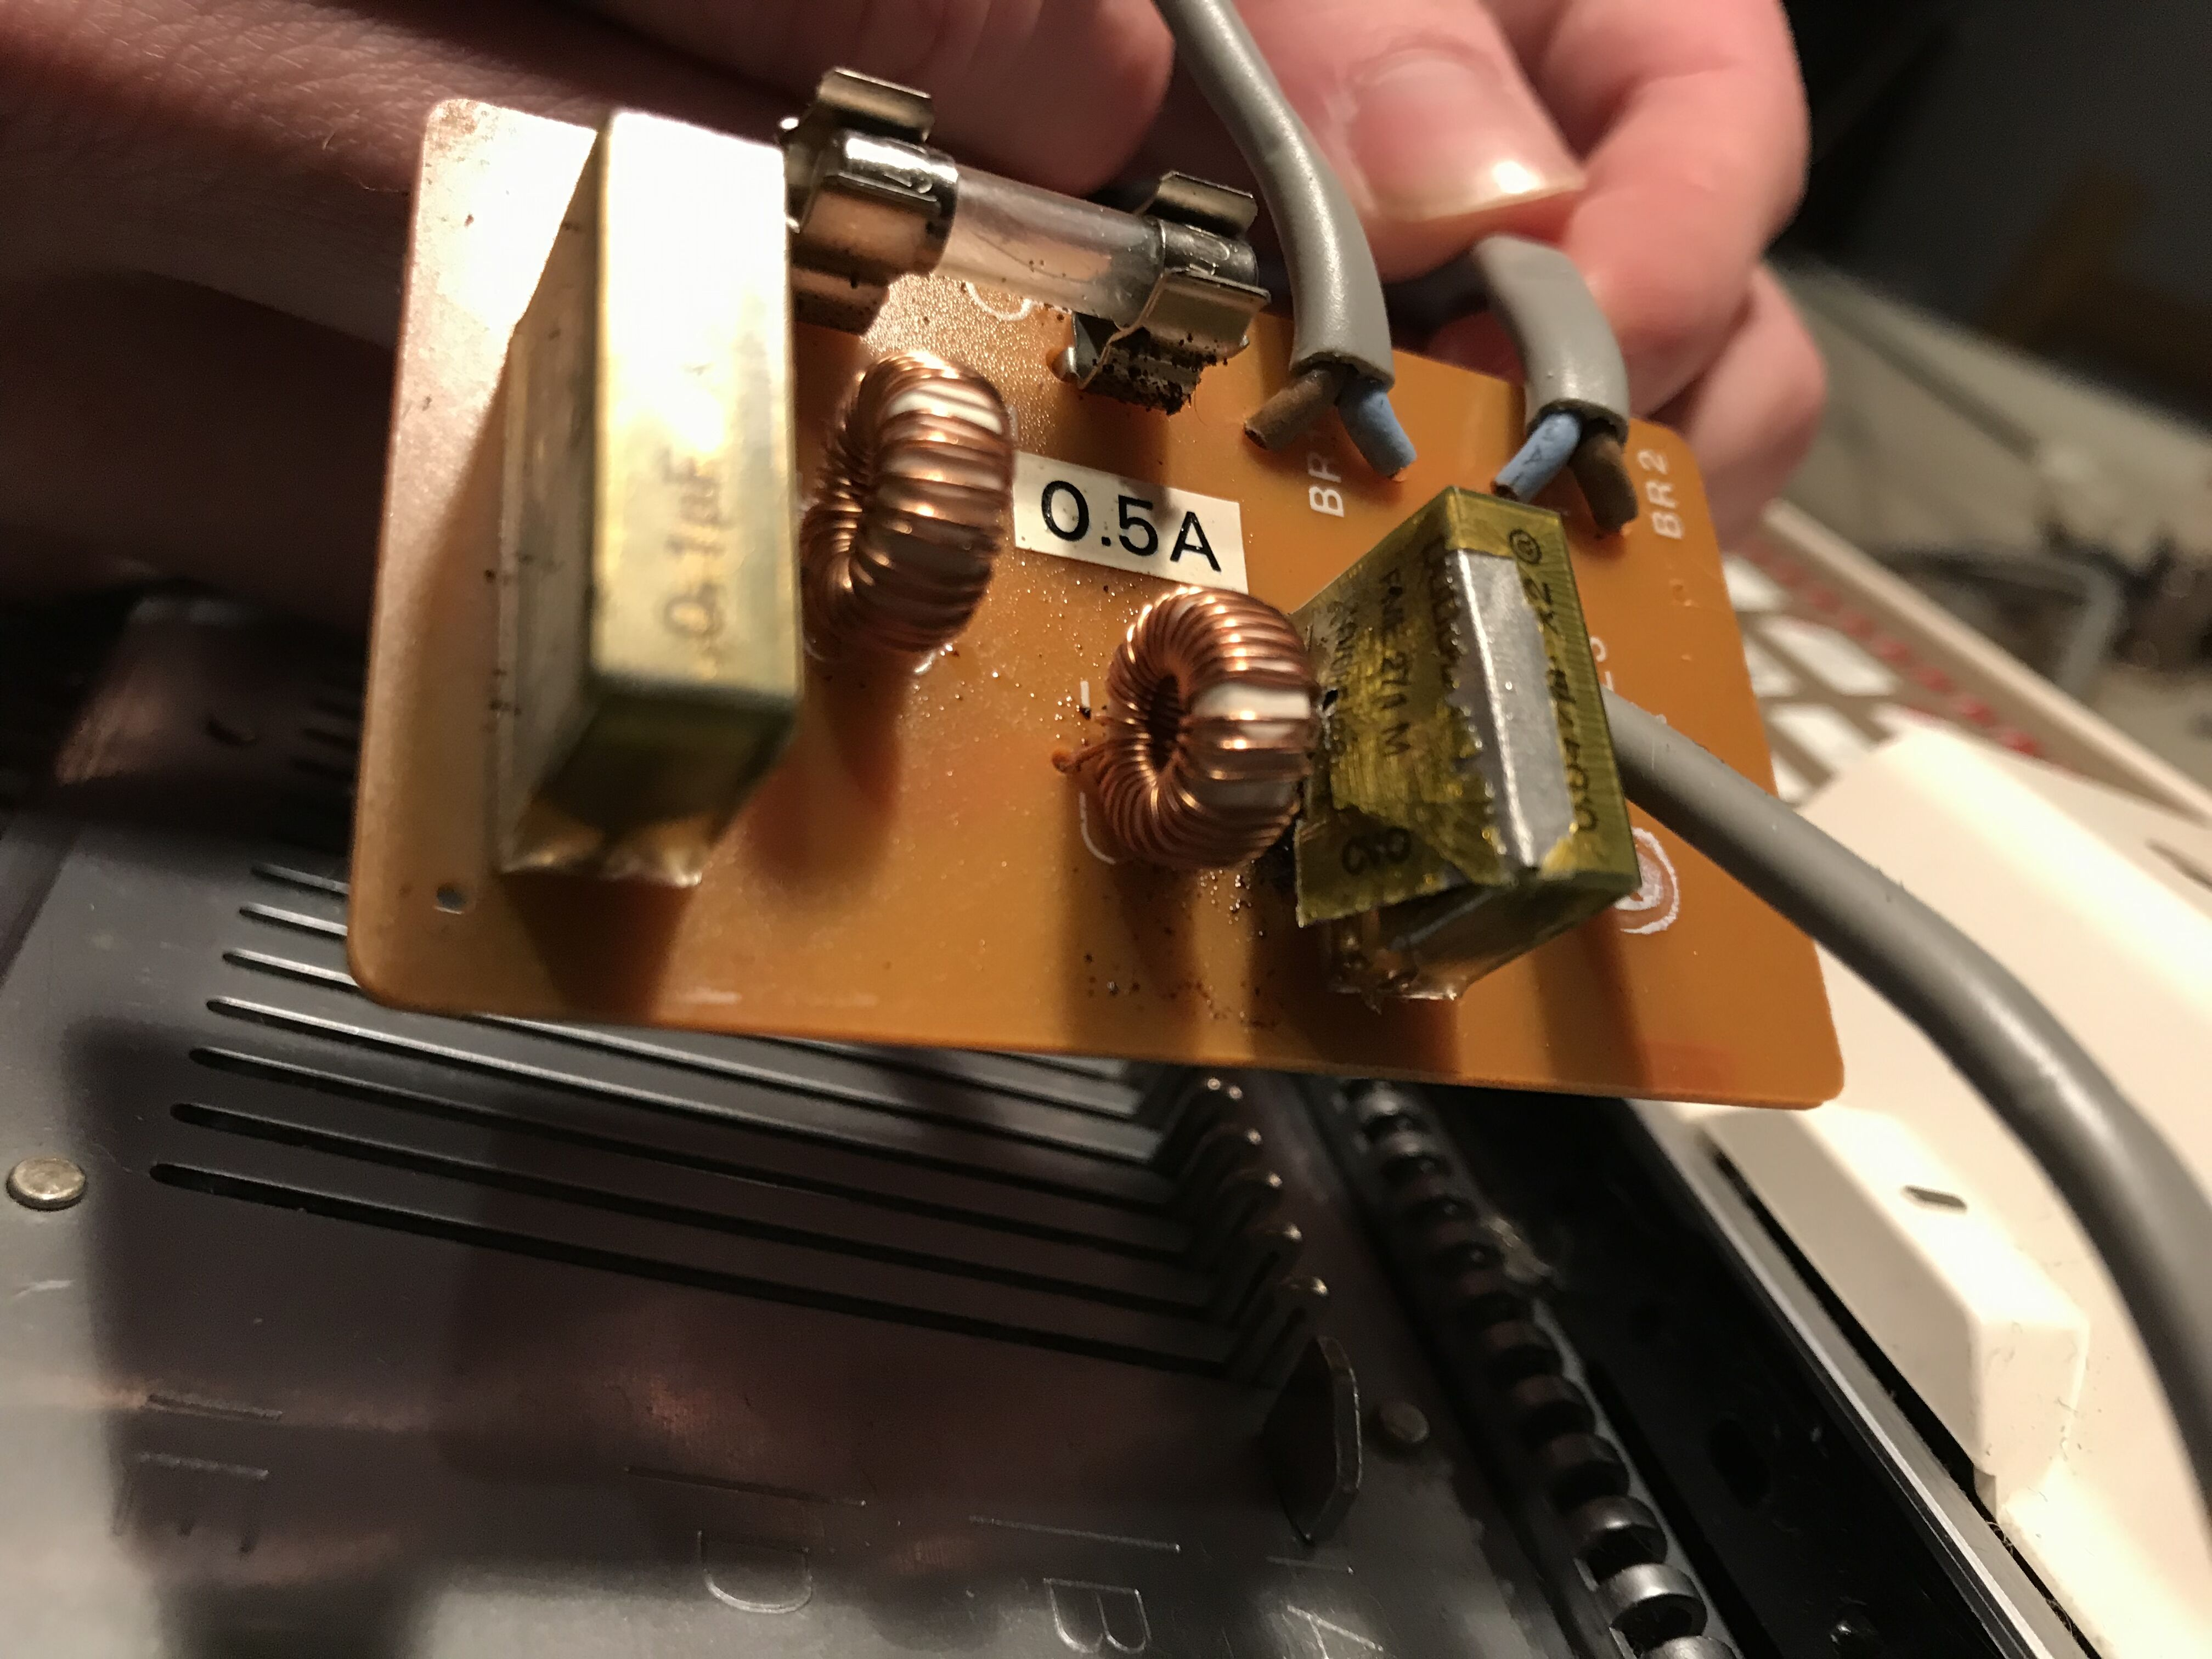
\includegraphics[width=0.7\textwidth]{./images/exploded-capacitor.png}
        \caption{fubar}
    \end{figure}
\end{frame}

\begin{frame}{progress}
    \begin{enumerate}
        \item project name (x)
        \item github repos (x)
        \item logo (x)
        \item knit manually (x)
        \item power on ... FAILED\pause
        \item repair...
    \end{enumerate}
\end{frame}

%% images
% - repairing

\begin{frame}{progress}
    \begin{enumerate}
        \item project name (x)
        \item github repos (x)
        \item logo (x)
        \item knit manually (x)
        \item power on ... FAILED
        \item repair \pause (x)
    \end{enumerate}
\end{frame}

%% image
% - works again

\begin{frame}{next steps}
    \begin{enumerate}
        \item knit more manually
        \item understand protocol better
        \item driver implementation
        \item image processing
    \end{enumerate}
\end{frame}

\end{document}
